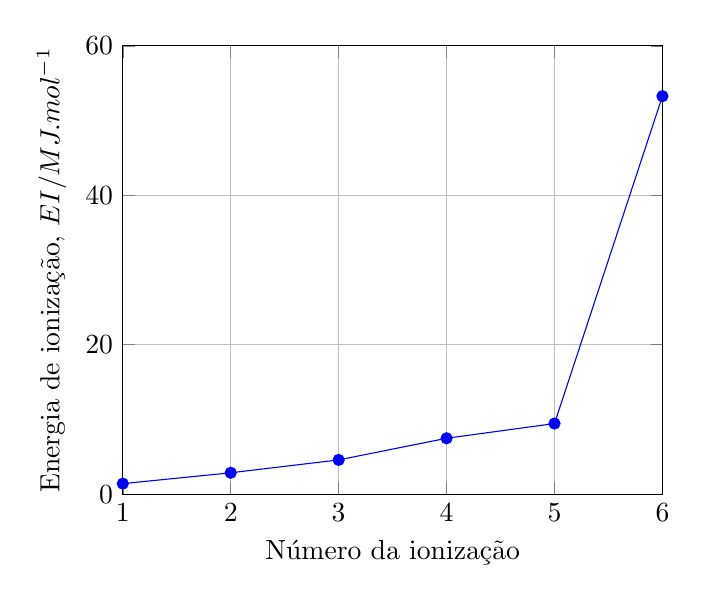
\begin{tikzpicture}
    \begin{axis}
        [
            grid=major,
            xlabel = {Número da ionização},
            ylabel = {Energia de ionização, $EI/\si{MJ.mol^{-1}}$},
            xmax=6, xmin=1, ymin=0, ymax=60
        ]
    \addplot[mark=*,color=blue] coordinates
        {
            (1, 1.402)
            (2, 2.856)
            (3, 4.578)
            (4, 7.475)
            (5, 9.444)
            (6, 53.266)
        };
    \end{axis}
\end{tikzpicture}